%%%%%%%%%%%%%%%%%%%%%%% file template.tex %%%%%%%%%%%%%%%%%%%%%%%%%
%
% This is a general template file for the LaTeX package SVJour3
% for Springer journals.          Springer Heidelberg 2010/09/16
%
% Copy it to a new file with a new name and use it as the basis
% for your article. Delete % signs as needed.
%
% This template includes a few options for different layouts and
% content for various journals. Please consult a previous issue of
% your journal as needed.
%
%%%%%%%%%%%%%%%%%%%%%%%%%%%%%%%%%%%%%%%%%%%%%%%%%%%%%%%%%%%%%%%%%%%
%
% First comes an example EPS file -- just ignore it and
% proceed on the \documentclass line
% your LaTeX will extract the file if required
\begin{filecontents*}{example.eps}
%!PS-Adobe-3.0 EPSF-3.0
%%BoundingBox: 19 19 221 221
%%CreationDate: Mon Sep 29 1997
%%Creator: programmed by hand (JK)
%%EndComments
gsave
newpath
  20 20 moveto
  20 220 lineto
  220 220 lineto
  220 20 lineto
closepath
2 setlinewidth
gsave
  .4 setgray fill
grestore
stroke
grestore
\end{filecontents*}
%
\RequirePackage{fix-cm}
%
%\documentclass{svjour3}                     % onecolumn (standard format)
%\documentclass[smallcondensed]{svjour3}     % onecolumn (ditto)
\documentclass[smallextended]{svjour3}       % onecolumn (second format)
%\documentclass[twocolumn]{svjour3}          % twocolumn
%
\smartqed  % flush right qed marks, e.g. at end of proof
%
\usepackage[utf8]{inputenc}
\usepackage{longtable}
\usepackage{graphicx}
\usepackage{booktabs}
\usepackage{hyperref}
\usepackage[usenames,dvipsnames]{color}
\usepackage{natbib}
\usepackage{lscape}
\usepackage{float}
\usepackage{rotating}



%
 \usepackage{mathptmx}      % use Times fonts if available on your TeX system
%
% insert here the call for the packages your document requires
%\usepackage{latexsym}
% etc.
%
% please place your own definitions here and don't use \def but
\newcommand{\jri}[1]{{\small \textcolor{blue}{\bf #1}}}
\newcommand{\pb}[1]{{\small \textcolor{Tan}{\bf #1}}}
% supplement numbering here i come!
\newcommand{\beginsupplement}{%
        \setcounter{table}{0}
        \renewcommand{\thetable}{S\arabic{table}}%
        \setcounter{figure}{0}
        \renewcommand{\thefigure}{S\arabic{figure}}%
 }

%
% Insert the name of "your journal" with
 \journalname{Chromosoma}
%
\begin{document}

\title{Diversity and evolution of centromere repeats in the maize genome%\thanks{Grants or other notes
%about the article that should go on the front page should be
%placed here. General acknowledgments should be placed at the end of the article.}
}
%\subtitle{Do you have a subtitle?\\ If so, write it here}

\titlerunning{Centromere repeats in the maize genome}        % if too long for running head

\author{Paul Bilinski \and Kevin Distor \and Jose Gutierrez-Lopez \and Gabriela Mendoza Mendoza \and Jinghua Shi \and R. Kelly Dawe \and Jeffrey Ross-Ibarra}

%\authorrunning{Short form of author list} % if too long for running head

\institute{Paul Bilinski : Kevin Distor : Jose Gutierrez-Lopez : Gabriela Mendoza Mendoza : Jeffrey Ross-Ibarra\at
              Department of Plant Sciences, UC Davis\\
              Davis, California, 95616
              \and
              Jeffrey Ross-Ibarra\at
              The Genome Center and Center for Population Biology, University of California\\
              Davis, California, 95616\\
              \email{rossibarra@ucdavis.edu}           %  \\
              \and
              Jose Gutierrez-Lopez\at
              Department of Natural Resources and the Environment
              University of New Hampshire\\
              Durham, New Hampshire, 03820
%             \emph{Present address:} of F. Author  %  if needed
           \and
           Jinghua Shi : R. Kelly Dawe\at
           Department of Plant Biology, University of Georgia\\
	  Athens, Georgia, 30602
}

\date{Received: date / Accepted: date}
% The correct dates will be entered by the editor
\maketitle

\begin{abstract}

Centromere repeats are found in most eukaryotes and play a critical role in kinetochore formation.  
Though centromere repeats exhibit considerable diversity both within and among species, little is understood about the mechanisms that drive centromere repeat evolution.  
Here, we use maize as a model to investigate how a complex history involving polyploidy, fractionation, and recent domestication has impacted the diversity of the maize centromeric repeat CentC.  
We first validate the existence of long tandem arrays of repeats in maize and other taxa in the genus \emph{Zea}.  
Although we find considerable sequence diversity among CentC copies genome-wide, genetic similarity among repeats is highest within these arrays, suggesting that tandem duplications are the primary mechanism for the generation of new copies.  
Nonetheless, clustering analyses identify similar sequences among distant repeats, and simulations suggest that this pattern may be due to homoplasious mutation.  
Although the two ancestral subgenomes of maize have contributed nearly equal numbers of centromeres, our analysis shows that the majority of all CentC repeats derive from one of the parental genomes, with a even stronger bias when examining the largest assembled contiguous clusters.  
Finally, by comparing maize with its wild progenitor teosinte, we find that the abundance of CentC likely decreased after domestication, while the pericentromeric repeat Cent4 has drastically increased. 

\keywords{Centromere \and Evolution \and Subgenome}
% \PACS{PACS code1 \and PACS code2 \and more}
% \subclass{MSC code1 \and MSC code2 \and more}
\end{abstract}

\section*{Introduction}
\label{intro}
In spite of the rapid growth in the number of sequenced genomes,  centromeres remain poorly understood and relatively cryptic due to their highly repetitive content.
Centromere repeats are highly diverse across taxa and their turnover appears to be very rapid \citep{Melters2012}. 
However, little is known about the genetic mechanisms that produce centromere repeat diversity.
Domesticated maize (\emph{Zea mays} ssp. \emph{mays}) has a high quality genome assembly \citep{Schnable2009} including complete sequence of two centromeres \citep{Wolfgruber2009}, and the breadth of research into maize centromeres makes it one of the best systems to investigate the processes governing centromere repeat evolution.

Maize centromeres are comprised primarily of the 156 bp satellite repeat CentC and the CRM family of retrotransposons.
Both repeats interact with kinetochore proteins such as CENH3 \citep{Wolfgruber2009, Zhong2002} and show variation in abundance across taxa \citep{Albert2010}.
While considerable effort has gone to investigating the molecular function of maize centromere repeats \citep{Ananiev1998B, Nagaki2003, Wolfgruber2009}, we know comparatively little about the evolution responsible for producing the current sequences. 
CRM elements are better understood, including the age and insertion preferences of different CRM families \citep{Wolfgruber2009, Sharma2008, Sharma09052014}.
In contrast, no in-depth characterization of the genetic diversity of centromere repeats in the maize genome exists.  

In this paper, we describe the patterns of diversity of centromere repeats across the maize genome.  
We investigate whether the differential ancestry of maize centromeres \citep{Wang2012} has led to chromosome-specific variation of CentC similar to that seen in other species \citep{Kawabe2005, hall2005differential, macas2010global} and how genetic relatedness among individual CentC repeats varies spatially across the genome.
We find that CentC copies do not form genetic groups consistent with ancient whole genome duplications or chromosome specificity, despite most of the large arrays of CentC originating from only one of the ancestral subgenomes of maize.
We show higher genetic similarity of CentC repeats within clusters, indicating the predominance of tandem duplications in the formation of new CentC copies.
Lastly, we use low coverage sequencing and cytological data to show that domesticated maize has less CentC than its wild relatives.

\section*{Methods} 
\label{methods}

\subsection*{CentC Repeat Identification and Diversity}

We downloaded 218 previously annotated CentC sequences \citep{Ananiev1998B, Nagaki2003} from Genbank.  
We then searched the B73 maize reference genome (5b60, \url{www.maizesequence.org}) with megaBLAST \citep{McGinnis2004} using the 218 annotated CentCs as a reference, keeping the longest hit with a length of over 140 bp and a minimum bit score of 100.
In this analysis, we defined CentC copies as tandem if their start locations were within 1000 bp.
	
All 12,162 CentC sequences were aligned using 7 iterations of Muscle \citep{Edgar2004} with default parameters.
A Jukes-Cantor distance matrix of all sequences was calculated with PHYLIP (\citep{Felsenstein1989} \url{http://evolution.genetics.washington.edu/phylip.html}), and an unrooted neighbor joining tree was built based on the distance matrix.  
	
We used principle coordinate analysis (PCoA) to cluster CentC variants based on their genetic distances. 
Eigenvalues from the PCoA were used to determine the number of statistically significant clusters using the Tracy-Widom distribution \citep{Patterson2006}.  
	
We employed the software SpaGeDi (\citep{Hardy2002}\url{http://ebe.ulb.ac.be/ebe/Software.html}) to estimate the spatial autocorrelation of sequence similarity of CentC repeats in the completely sequenced centromeres 2 and 5.
We calculated Moran’s I statistic using Jukes-Cantor genetic distance and measures of physical distance between CentC repeats in base pairs.
Confidence intervals for the values of I were estimated by 20,000 random permutations of the physical distances.  
	
Statistical analyses were performed in R with the packages ape \citep{Paradis2004} and RMTstat \citep{Perry2009}.  
We compared clusters to chromosome of origin and syntenic maps of maize ancient tetraploidy \citep{Schnable2011} to determine if the genetic history of maize left a footprint on CentC similarity.

\subsection*{Read Mapping and Genome Size Correction}
	
We mapped Illumina reads from a broad panel of \emph{Zea} species \citep{Chia2012,Tenaillon2011}  to a reference consisting of the full complement of 12,162 CentC variants identified in the B73 genome.  
We also used previously published sequence from whole genome chromatin immunoprecipitation (ChIP) \citep{Wolfgruber2009, Wang2013} using CenH3.  Reads were mapped with  Mosaik v1.0 (\url{https://code.google.com/p/mosaik-aligner/}). 
We first optimized mapping parameters by relaxing mapping stringency and evaluating the number of successfully mapped reads with each combination.  
Consistent with parameters from previous studies mapping reads to repetitive elements \citep{Tenaillon2011}, we required homology to remain at a minimum of 80\%.  
For other non-default parameters, we permuted over many values of hash size, alignment candidate threshold,  percent of read aligning, and maximum number of hash positions per seed to find a combination that produced believable alignments.  
We selected an optimum combination of parameters just below the parameters where we observed a large increase in the total number of reads aligning (Figure \ref{Supp_MPS}).
Our final set of parameters for tandem repeats used an initial hash size of 8, an alignment candidate threshold of 15 bases, 20\% of mismatching bases, a minimum of 30\% overlap to the reference, and stored the top 100 hits for alignment.  
After reads were mapped, we calculated the percentage of total reads hitting the given reference and multiplied this value by the relative genome size of each accession as reported in \citet{Chia2012} and \citet{Tenaillon2011}. 
The total number of reads mapping did not change drastically when using one random copy of CentC versus the full AGPv2 reference, suggesting that our parameters are sufficiently broad to capture genome-wide CentC abundances.  
Because library preparation has an effect on estimates of repeat abundance (see results), we only used individuals from maize HapMap v2 \citep{Chia2012} with libraries prepared using identical methods.
	
We used a different set of mapping parameters for long repeats such as transposable elements.  
Previous studies \citep{Schnable2009} estimated that approximately 85\% of maize genome derives from transposable elements.  
Using the short read libraries from \citet{Tenaillon2011}, we selected parameters so that approximately 85\% of the library mapped to the maize transposable element database (\url{www.maizetedb.org}) with a minimum homology of 80\%.  
The final parameters for TEs were a hash size of 10, alignment candidate threshold of 11, 80\% homology excluding non-aligned portions of the read, and a 30\% minimum overlap.

We designed a simulation to estimate the accuracy of our measurements of CentC content (code available at: \url{https://github.com/kddistor/dnasims}).  
In short, our simulations altered the copy number of CentC repeats over a region of fixed length (10 Mb), changing the percentage of the genome deriving from the repeat.  
Illumina reads were simulated from each of the DNA strings and mapped using our pipeline.  These simulations showed that our pipeline captured relative differences in abundance well, but underestimated total abundance of CentC.  
We found that our pipeline could accurately capture differences of 0.05\% change in CentC abundance, suggesting that larger differences are likely to be biologically real (Figure \ref{Supp_Accuracy}).  

\subsection*{Simulation of homoplasious mutations}

In order to better understand patterns of diversity at CentC, we performed simulations to test the likelihood of homoplasious mutations (i.e. independent mutations occurring at the same position in two different CentC repeats). 
Our simulation (code available at: \url{https://github.com/paulbilinski/CentC_Analyses/tree/master/Diversity_sims}) assumed that CentC has been evolving for 1 million years since the divergence of maize and \emph{Tripsacum} \citep{Ross-Ibarra2009}, a closely related genus whose centromere repeat shares a large amount of homology \citep{Melters2012}.  
We assumed a constant copy number, a mutation rate of $3 x 10^{-8}$ per generation \citep{clark2005estimating}, and one generation per year.  

\subsection*{PacBio Sequencing}
	
Library preparation and sequencing was performed according to the methods described in \citep{Melters2012}.  
Using those protocols, we sequenced one individual from \emph{mays}, \emph{mexicana}, \emph{parviglumis}, and \emph{Z. luxurians} with Pacific Biosciences (Pacific Biosciences, Menlo Park, CA) technology. 
Approximately 200 Mb of reads were produced from each cell, and reads with length greater than 600 bp were retained for analysis of tandem CentC content using BLAST (Table \ref{supp.pacbio}).  
CentC copies were considered tandem if the read had 4 CentC copies each within 300 bp of each other. 

\subsection*{FISH}

Fluorescent in situ hybridization (FISH) was carried out as described in \citet{kato2004paint} for a B73 by \emph{Z. luxurians} hybrid) and \citet{Shi2010} for a B73 by \emph{Z. parviglumis} hybrid. 

\section*{Results}
\label{results}

\subsection*{Centromere repeats in the maize genome}

We found a total of 12,162 CentC copies in the maize reference genome and unassembled BACs.  
Of these, 8,259 were unique over their full length.
While centromeres 2 and 5 are the only chromosomes with high confidence sequencing of CentC copies, the levels of diversity observed on these two chromosomes is comparable to the rest of the genome (data not shown), suggesting that current assemblies of CentC sequence may estimate sequence variation with some accuracy.
No CentC sequence occurred more than 10 times in the genome, and the vast majority ($>$75\%, Table \ref{supp.occurence}) of non-unique CentC variants occurred only twice.  
Of the 2,266 non-unique CentC sequences, only 3 were tandem, identical duplicates.  
Nearly all of the 10,639 CentC copies on chromosomes 1-10 are found in clusters; only 14 occurred as solo copies.  
Clusters varied in width from single CentC copies to 84 Kb with a mean of $\sim$7 Kb ($\sim$45 CentC copies). 
Chromosomes varied greatly in CentC copy number, although centromere assemblies for all of the chromosomes are not complete.   
For example, CENH3-ChIP sequence from an oat-maize addition line with one maize chromosome \citep{kynast2001} has many reads that map to the unassembled BACs (Table \ref{supp.gaby}).  
In particular, chromosome 6 has many more reads aligning to the unassembled BACs than it did to its own centromere repeats, suggesting a particularly incomplete assembly.  
Examining total repeat number, chromosome 7 had the most CentC, with 3,200 copies, while chromosome 6 had the fewest with 32 copies.

We used long-read Pacific Biosciences sequencing to verify that most CentC is in tandem arrays. 
We sequenced whole genome ($\sim 0.1$X) libraries from 4 \emph{Zea} taxa.  
In spite of the low coverage, we recovered reads containing CentC sequence from all four taxa (Table \ref{supp.pacbio}).  
In one 6.7 Kb read from the maize reference line B73, for example, we identified approximately 40 independent CentC copies in tandem, and similar arrays were seen in all four \emph{Zea} species analyzed.  
These results show that overall structure of the repeats has been maintained for the approximately 140,000 years since the \emph{luxurians}-\emph{mays} divergence \citep{Hanson1996,  Ross-Ibarra2009} and that a majority of CentC is found in tandem arrays (Table \ref{supp.pacbio}).

We then identified how many large clusters of CentC were retained from each of the two parental genomes that comprise the extant maize genome, referred to here as subgenome 1 and subgenome 2 (Figure \ref{circos}).  
Previous work identified the parental genome for individual chromosomal segments \citep{Schnable2011} and centromeres \citep{Wang2012}, with centromeres 1, 2, 5, 7, 9, and 10 deriving from subgenome 1 and 3, 4, 6, 8 from subgenome 2.  
Due to the maize iMap resource \citep{zhou2009single}, we believe large clusters are less likely to be misplaced within the genome.
Therefore, we focused our analyses on the 52 clusters $>$10 Kb in length (Supplementary Fig \ref{Supp_clusterhist}).
We assign clusters to a subgenome if they are flanked by two regions identified as originating from the same  subgenome.  
Thirty-eight of these clusters could be assigned to subgenome 1 (out of 43 assignable).
If we restrict the analysis to clusters  $>$20 Kb with clear assignment to one subgenome, all 16 clusters were found in subgenome 1.  
Even correcting for the genome-wide overrepresentation of subgenome 1 (64.7\% of assigned base pairs), these results suggest a strong inequality in the origin of large CentC clusters (Fisher's exact test, $p<0.005$ for both 10 Kb and 20 Kb clusters).
One cluster $>$20 Kb falls within an unassigned region on chromosome 3.
This difference between the subgenomes is robust to different criteria of cluster size and distance (Table \ref{tab:suppvartandem}).

\begin{figure}
% For two-column wide figures use
% Use the relevant command to insert your figure file.
%  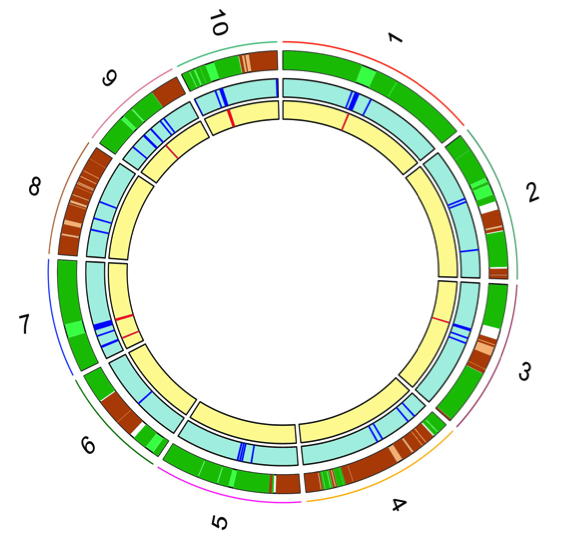
\includegraphics[width=0.75\textwidth]{circos.png}
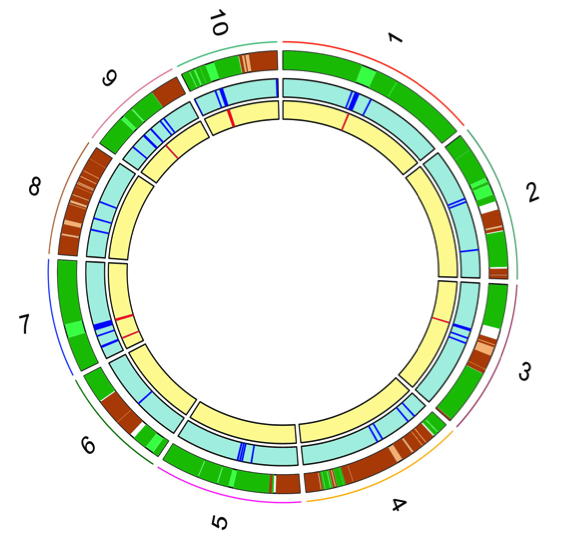
\includegraphics{Fig1_circos}
\caption{CentC repeat location in relation to the maize subgenomes.  The outer ring depicts chromosomal assignment to the two subgenomes, with higher confidence regions in darker colors.  Green corresponds to subgenome 1, brown to subgenome 2.  Breakpoints between the subgenomes remain uncolored to indicate uncertainty. The middle ring, shaded in blue, displays the locations of all CentCs across the genome.  The inner ring, shaded in yellow, displays the locations of all CentC clusters greater than 20 Kb in length}
\label{circos}    
\end{figure}

Previous studies have also described the Cent4 repeat, a tandem pericentromeric repeat that occurs primarily on chromosome 4 \citep{Page2001}. 
Available evidence does not point to any centromere function for Cent4: CenH3 chromatin immunoprecipitation data \citep{Wolfgruber2009, jin2004maize} show no significant over-representation of Cent4 compared to five known non-centromeric TE’s, fiber FISH shows clear separation of Cent4 from centromeric repeats \citep{jin2004maize} and Cent4 probes lag behind CentC probes in cell division, suggesting that they are not found in the kinetochore \citep{Jiang2002, jin2004maize}. 
BLAST analyses of Cent4 sequences from Genbank revealed high homology to the poorly characterized LTR retrotransposon RLX\_sela that was previously shown to be associated with heterochromatic  knobs \citep{Tenaillon2011, Chia2012}, but Cent4 lacks any of the protein sequences necessary for autonomous transposition, such as GAG and POL complexes.  
But while previous work in rice has documented the presence of nonautonomous LTR retrotransposons  in or near the centromere \citep{Jiang2002}, RLX\_sela also appears to be missing the necessary primer binding sites that would distinguish it as a nonautonomous TE, suggesting that it may be a TE-derived tandem repeat unique to the pericentromere of chromosome 4. 

\subsection*{Relatedness of CentC in the maize genome}

CentC copies in the maize genome exhibit tremendous diversity: the overall pairwise identity in our alignment was only 65\%, and $\sim$98\% of sites in the alignment had at least 2 variants.  
Such diversity led us to ask whether genetic groups of CentC variants could be distinguished. 
We performed principle coordinate analyses (PCoA) from a genetic distance matrix estimated from our alignment, and assigned individual repeats to  genetic clusters following the approach of \citet{Patterson2006}.  
We found 58 significant clusters, but observed no pattern of groupings that revealed chromosome specificity of CentC’s or the impact of historical tetraploidy (Figure \ref{pcoa}; Table \ref{long}).

\begin{figure}[h]
\centering
% For two-column wide figures use
% Use the relevant command to insert your figure file.
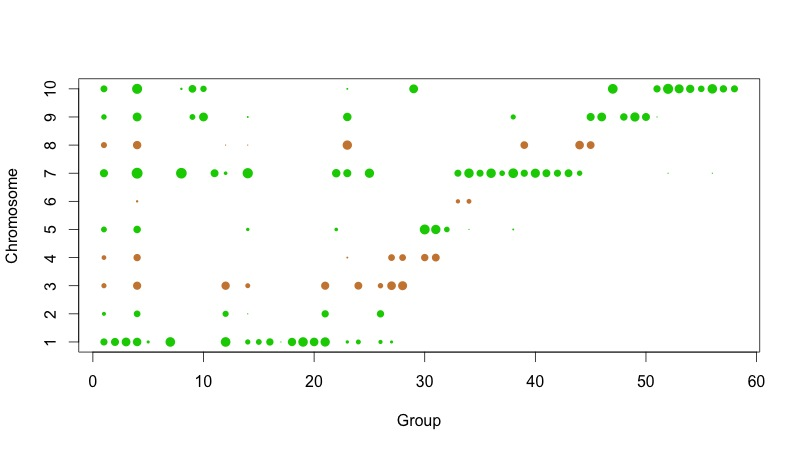
\includegraphics[width=1\textwidth]{Fig2_TWgroups}
\caption{Presence of CentC in each of the hierarchical groups.  The 58 clusters found to be statistically significant in forming genetic groups are represented on the x-axis and chromosome of origin on the y-axis. The size of each point is proportional to the log number of sequences in that group on that chromosome. CentC counts from chromosomes whose centromeres were derived from subgenome 1 are colored green and those from subgenome 2 are colored brown 
}
\label{pcoa}    
\end{figure}

The tandem nature of CentC suggests it increases in copy number through local duplications that produce initially identical copies.  
Tandem duplications can occur through a variety of means, including slippage of the DNA polymerase or recombination that could lead to unequal crossing over or gene conversion.
Tandem duplication predicts that  clusters of CentC should be more closely related than CentC from different clusters.  
Comparisons of genetic and physical distance among CentC repeats on chromosomes 2 and 5 shows that average genetic similarity is highest within clusters (Figure \ref{heatmap}), revealing significant spatial autocorrelation of CentC variants over distances up to 10-50 Kb (Figure \ref{Supp_SpagediChr02} and \ref{Supp_SpagediChr05}).

\begin{figure}[h]
\centering
% For two-column wide figures use
% Use the relevant command to insert your figure file.
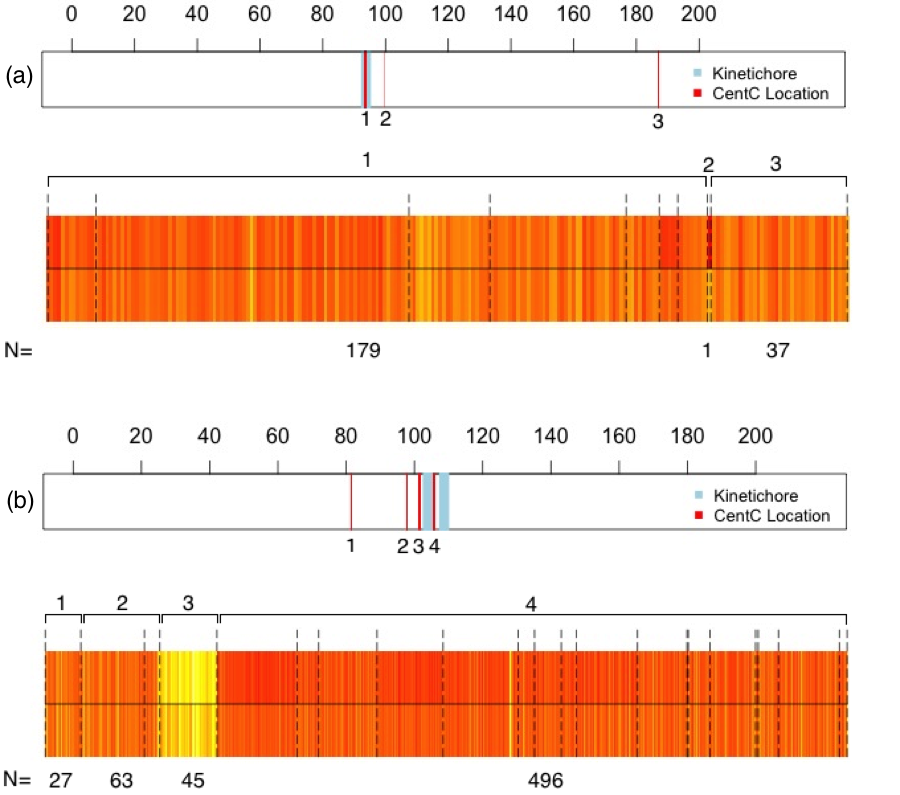
\includegraphics[width=1\textwidth]{Fig3_Heatmap}
\caption{CentC physical location and genetic relatedness for (a) chromosome 2 and (b) chromosome 5.  On the physical map above, red lines show locations of numbered CentC clusters and blue blocks show the location of the active kinetochores.  Scale bar is in Mb.  Below each physical map is shown a heatmap of genetic relatedness of each CentC to (top row) other copies within its island of tandem repeats delineated by dotted lines and (bottom row) all other copies on the chromosome.  Darker colors indicate higher relatedness.  The total number of CentC in each cluster is shown below the map
}
\label{heatmap}    
\end{figure}

The decreased genetic distance among CentCs in local clusters on chromosome 2 and 5 suggest that many of the genetic groupings discovered in our genome-wide analysis should correspond to local clusters of repeats. 
However, repeats within individual clusters are frequently found in different genetic groups as defined by principle coordinate analysis (Figure \ref{pcoa}).
We observed multiple pairs of CentC which occur in the same genetic cluster in spite of being separated on the completely sequenced centromeres 2 and 5, suggesting that our result is not simply an artifact of errors in assembly.
A comparison of shared mutations across all pairs of CentC sequences reveals a potential explanation.  
Of the $\sim 74$ million possible pairs,  approximately 6 million share $\geq 2$ mutations different from the genome-wide consensus, causing CentC copies to group with sequences that share mutations irrespective of their physical distance.  
Comparing several triplets at random from our alignment confirms that two sequences in one PCoA assignment share greater pairwise identity than two sequences adjacent to one another in different PCoA groups.  
A simple forward simulation (see Methods) suggests this pattern could be due entirely to homoplasy rather than long-distance movement of CentC repeats.  
By stochastically applying mutations to an initially homogeneous group of repeat sequences, we find that plausible parameter values produce $\sim 10$ million pairs of repeats sharing $\geq 2$ mutations.

\begin{figure}
% For two-column wide figures use
% Use the relevant command to insert your figure file.
\centering
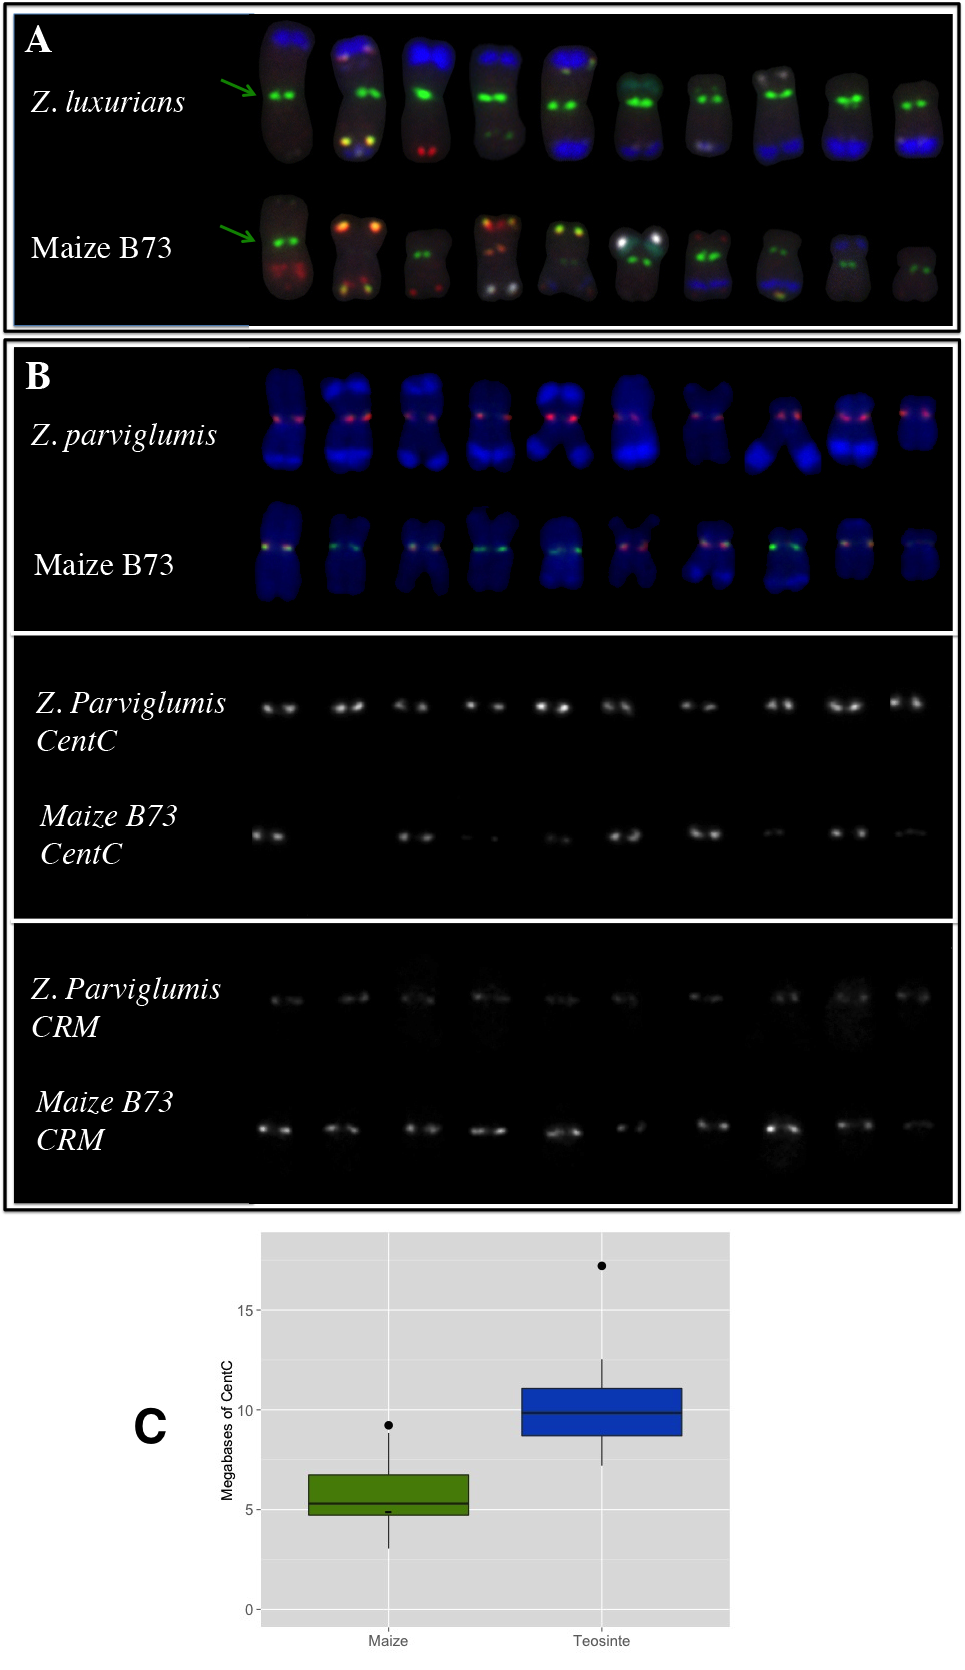
\includegraphics[width=1\textwidth]{Fig4_kelly2}
\caption{(a) FISH analysis of a single individual heterozygous for B73 and \emph{Zea luxurians} (GRIN accession PI422162).
Chromosomes, ordered from 1 (left) to 10 (right), were hybridized with the \citet{kato2004paint} probe cocktail. 
Green shows CentC and a 4-12-1 subtelomere repeat, blue the 180 bp knob repeat, red the abundant TAG microsatellite and another subtelomeric repeat, white the TR1 knob repeat, orange the Cent4 repeat, yellow the 5S rDNA repeat, and aqua shows the Nucleolus Organizer Region.
The green signals at the primary constrictions (arrows) are CentC.
Note that \emph{Z. luxurians} has far brighter CentC signals.
This image was graciously provided by Patrice Albert.
(b) FISH analysis of a single individual heterozygous for B73 and \emph{Z. parviglumis}(GRIN accession PI566687).
Chromosomes were hybridized with the \citet{Shi2010} probe cocktail showing CentC in red and CRM2 in green. 
Each separate probe is shown separately below the two-color image, highlighting that CentC is more abundant in \emph{Z. parviglumis} and CRM2 is more abundant in maize. 
(c)  Mb of CentC in genomic libraries of maize and teosinte. 
Box plots show data from \citet{Chia2012}. 
Points show data for maize inbred B73 and the teosinte \emph{Z. luxurians} from \citet{Tenaillon2011}. For comparison, the data point of maize inbred B73 in \citet{Chia2012} is shown with a tick mark on the box plot.
}
\label{abundance}    
\end{figure}

\subsection*{Variation of CentC abundance in \emph{Zea}}

Shotgun sequence data from the maize HapMap v2 \citep{Chia2012}, reveals a significantly greater abundance of CentC in teosinte than in domesticated maize (p$<0.01$; Figure \ref{abundance}).   
Further support for differences between maize and its wild relatives comes from additional  sequence  from \emph{Z. luxurians} \citep{Tenaillon2011}.  
Analysis of these data find nearly twice as much CentC in \emph{Z. luxurians} as the maize inbred B73.  
To corroborate these results, we performed fluorescent in-situ hybridization of F1 crosses between inbred maize and teosinte to determine if cytological observations agreed with our sequencing findings.   
FISH data supports our observation that the teosintes \emph{parviglumis} and \emph{Z. luxurians} have more CentC than inbred maize (Figure \ref{abundance}).
Using whole genome shotgun PacBio long reads, we further investigated the overall structure of repeats across the different \emph{Zea} species.
Percentages of the libraries showing tandem repeats were also higher in PacBio sequences from three teosinte compared to B73 (Table \ref{supp.pacbio}).

\section*{Discussion}
\label{discussion}

Our analysis of centromere repeat diversity across the maize genome identifies thousands of copies exhibiting tremendous diversity. 
But while we can cluster the repeats into groups of related sequences, these groups have little relation to current or ancient maize chromosomes (Figure \ref{pcoa}).
We find no evidence of chromosome specific repeats as observed in \emph{Arabidopsis} species \citep{Kawabe2005, Pontes2004}, suggesting the presence of a mechanism that homogenizes repeats across centromeres on different chromosomes.
Although we believe our results relatively robust to assembly errors, misplaced BACs and collapsed tandem copies almost certainly occur in the maize  reference genome and may influence our assessment of chromsome-wide patterns.
We further verify that Cent4, once thought to be a chromosome-specific centromere repeat \citep{Page2001}, appears to be a poorly characterized tandem repeat or nonautonomous retroelement, but is not associated with the centromere.  

We find that virtually all the large arrays of CentC in the maize  genome derive from one of the two ancestral genomes present in modern day \emph{Zea} (Figure \ref{circos}, Table \ref{tab:suppvartandem}).  
This biased ancestry mirrors differences in genic expression and deletion seen between the subgenomes  \citep{Schnable2011}. Higher deletion rates on subgenome 2 may explain our observation, but the finding of small regulatory RNA’s corresponding to centromeric repeats \citet{ReinhartBartel2002} in other taxa may suggest a more active mechanism behind the observed differences.  

%% STUFF JEFF MAY ADD TO DISCUSSION
%Phylogenetic analysis of centromere repeats from a large number of eukaryotes found that repeat abundance evolves more rapidly than expected under a simple model of brownian motion \ref{Melters2012}. 

%Therefore, it may be worthwhile to further investigate the potential correlation between centromere retention and gene expression as the phenomenon of higher expression of genes from one ancestor may be common across plants \citep{Cheng2012}.  There are several possible explanations for the differential contribution of subgenome 1 to the diversity of CentC in the extant maize  genome. Subgenome 2 may have had severely reduced quantities of CentC and therefore never contributed equally.  The CentC from subgenome 2 may have decayed rapidly and thus less of it remains.  Lastly, the CentC from subgenome 1 may have expanded in copy number since the allopolyploidy event.  Though we are unable to conclusively identify the reason, the lack of a large number of identical tandem duplicates  and lack of close proximity highest genetic relatedness pairs suggests that any large scale expansion of CentC has not been recent.  Also, CentC’s in subgenome 2 cluster do not appear to have accumulated excess mutation, suggesting that they are not decaying more rapidly than their subgenome 1 counterparts.  We therefore believe that it is most likely that the subgenomes had an unequal contribution of CentC at the formation of the allopolyploid, though more research about the ancient parents is required.  

% It is likely that our empirical value is lower than our simulated value because we assume that all CentC copies have existed since the divergence event, while it is much more likely that age is high variable across copies.  Provided with such a large percentage of copies sharing mutations through homoplasy, we posit that it is possible for homoplasy, in the form of repeated mutations in different CentC copies, to drive our PCoA groupings.

%!RELATEDNESS
Our sequence comparison of CentCs also enabled us to explore the relationship between genetic and physical distance among repeats.  
Using the well-assembled centromeres on chromosomes 2 and 5, we found spatial autocorrelation of relatedness among repeats, but also observed genome-wide that many CentC’s within an array fall into the same genetic cluster.
We observed no differences in genetic similarity when comparing clusters inside against cluster outside the active kinetochore.
Our observations are consistent with the simple idea that most repeats arise due to tandem duplication or related processes with similar outcomes such as small scale gene conversion or unequal crossing over.
Long distance transposition of CentC, while necessary to homogenize repeats across chromosomes \citep{Shi2010}, appears relatively uncommon.

One unusual result from our sequence comparison was the finding that pairs of CentC on different chromosomes share very high sequence similarity.  
Our simulations suggest that, under realistic assumptions about mutation rate and divergence time, such a pattern is possible due to homoplasious mutation alone.  
Roughly 80\% of the CentC repeats have their closest genetic relative on the same chromosome, as expected under a model of tandem duplication, but only 14\% of closest genetic pairs are found within 10 Kb of each other.
Though assembly errors may explain a portion of these relationships, we find several closest genetic pairs separated in the fully sequenced centromeres of chromosomes 2 and 5, suggesting our observation is biologically real.
We speculate that the vast majority of  CentC’s in the genome are thus a result of relatively old tandem duplications, and that sufficient time has occurred since duplication for rearrangements and mutations to break up patterns of identical tandem repeats.

%pairs investigating why a pair of chromosomes on two different chromosomes are each other closest genetic relative, we revealed that homoplasy in mutations is common across CentC variants.  We suggest that copies of CentC are sufficiently old within the genome that homoplasious mutations cause physically distant CentC’s to be highly genetically related.  Importantly, we also do not see PCoA group capturing full clusters across chromosomes in a way that would be consistent with retrotransposition. 


 % Given the lack of a genome wide pattern, we also wanted to investigate genetic relatedness on individual chromosomes.  We hypothesized that most copies of CentC arose from local duplication rather than transposition, and therefore the genetic distance between CentC’s would be lowest across CentC’s within a large tandem array.  \pb{This part is ugly, and needs help} From the reference genome, we chose to investigate chromosomes 2 and 5, since they have been sequenced from end to end, allowing for inferences about the relationship between diversity and physical proximity \citep{Wolfgruber2009}.  Furthermore, the role of the repeat arrays on chromosomes 2 and 5 appear very different, as the largest array on chromosome 2 interacts with the kinetochore, while no array on chromosome 5 does \citep{Wolfgruber2009}.  We find that repeats on chromosomes 2 and 5 are most highly genetically related to neighboring copies (Figure \ref{heatmap}).  This relationship was recapitulated in analyses using SpaGeDi, where CentC’s within approximately 10-50KB of one another were more genetically similar (Tables \ref{Supp_SpagediChr02} and \ref{Supp_SpagediChr05}).  Though we did not investigate the relationship between CentC location and genetic similarity on the other chromosomes due to incomplete sequencing of centromeres, we observe that many CentC’s within an array fall into the same  significant grouping in our Tracy-Widom clustering analysis, suggesting that high local similarity of CentC’s is a genome-wide phenomenon.  This local relatedness suggests that most CentC is evolving through tandem duplication and not a long distance mechanism such as transposition that had been previously suggested \citep{Shi2010}.  Concerning chromosomes 2 and 5, the higher local relatedness of all CentC clusters regardless of presence within the kinetochore suggests that CentC interaction with kinetochore proteins does not have a detectable change on their rates of evolution.


Previous cytogenetic work  identified  differences in centromere repeat content  between domesticated maize and its wild relatives \emph{Z. mays} ssp. \emph{parviglumis}, \emph{Z. mays} ssp. \emph{mexicana}, and \emph{Z. luxurians}  \citep{Albert2010} but was unable to quantify  differences. 
Our resequencing results show that while there is little difference in the distribution of CentC in tandem arrays, the absolute abundance of CentC has  decreased during domestication, and we verify this with FISH in two maize-teosinte hybrid individuals (Figure \ref{abundance}). 
%Decreasing CentC content during domestication contrasts with the apparent lack of change in transposable element abundance after controlling for genome size \citep{Chia2012}, suggesting that changes in CentC are not due to causes common to all repetitive sequence.
Variability in observed abundance of transposable elements \citep{Chia2012} suggests that the decrease seen in CentC is not due to causes common to all repetitive sequences.
The maize genome is smaller than its teosinte counterpart, largely due to differences in the abundance of heterochromatic knobs \citep{poggio1998}.  
\citet{Zhang2012} have postulated an adaptive relationship between centromere size and genome size based on an observed correlation between centromere size and genome size across a number of grass species.  
A model correlating centromere size to total genome size would propose that the decrease in CentC abundance seen post-domestication is due to selection for smaller active centromeres to complement the smaller overall genome size.
While our current data are insufficient to evaluate this conclusion, future work investigating differences in CentC content among maize landraces that vary in genome size \citep{poggio1998} may provide an opportunity to further test our hypothesis.  

In conclusion, our detailed study of centromere repeats in the B73 maize genome has highlighted differential contribution of subgenome, spatial autocorrelation along a chromosomes, and changes in abundance over the short time scale of domestication.  
Since maize lines show vast cytogentic variation, further work evaluating CentC evolution across multiple populations and multiple related species may shed additional light on the timing and causes of these changes.  

\begin{acknowledgements}
We wish to thank Pacific Biosciences for sequencing resources.  We thank Patrice Albert and James Birchler for providing the high-quality FISH image of the \emph{Z. luxurians} X B73 hybrid.  We thank Siddharth Bhadra-Lobo, Vince Buffalo, Anne Lorant, Gernot Presting, Lauren Sagara, Michelle Stitzer, and National Science Foundation summer exchange program interns Cesar Alvarez Mejia, Aurelio Hernandez Bautista for advice and helpful discussion. This project was funded by National Science Foundation grant IOS-0922703.
\end{acknowledgements}

% BibTeX users please use one of
\bibliographystyle{spbasic}      % basic style, author-year citations
%\bibliographystyle{spmpsci}      % mathematics and physical sciences
%\bibliographystyle{spphys}       % APS-like style for physics
\bibliography{refcentc}   % name your BibTeX data base

\newpage

\beginsupplement
\section*{Supplemental Material}

\begin{figure}[h!]
% For two-column wide figures use
% Use the relevant command to insert your figure file.
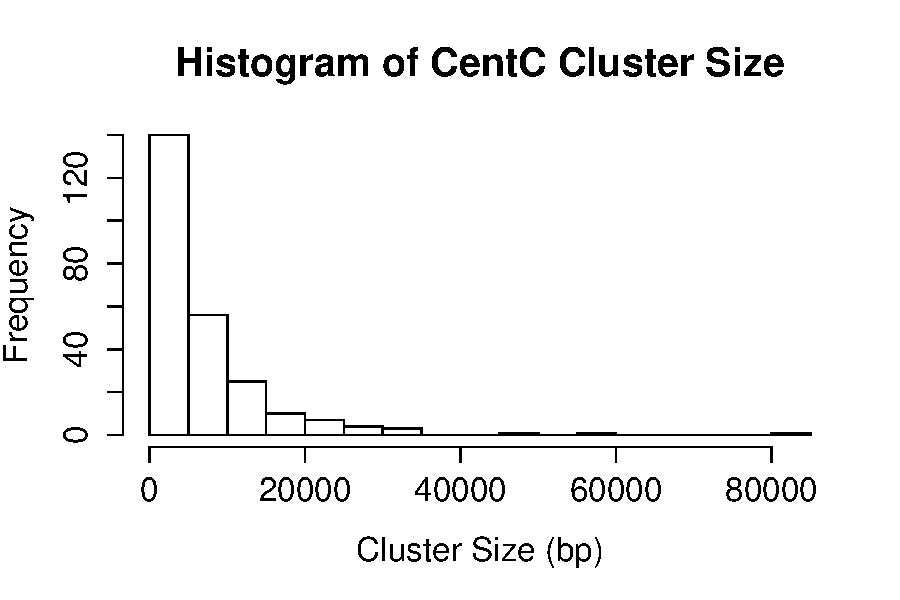
\includegraphics[width=1\textwidth]{Supp_clusterhist}
\setcounter{figure}{0}
\caption{CentC cluster size across all chromosomes.}
\label{Supp_clusterhist}    
\end{figure}

\begin{figure}[h!]
% For two-column wide figures use
% Use the relevant command to insert your figure file.
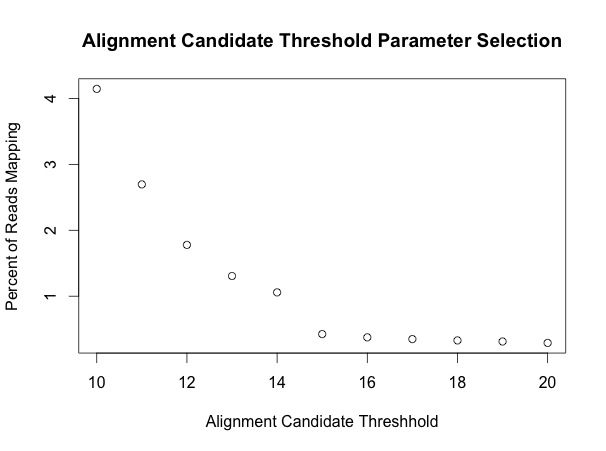
\includegraphics[width=1\textwidth]{Suppl_ACT_Seln.jpeg}
\caption{Parameter selection for Alignment Candidate Threshold (ACT) for Mosaik.  All other parameters were kept constant while ACT was changed.  ACT was the parameter for which a non-linear pattern was observed.  We selected to use an ACT of 15, the value for which we observed the greatest relative decrease between total percent mapping values.  The sharp change suggests that, at a lower ACT, we may be mapping a non-CentC element to our reference.}
\label{Supp_MPS}    
\end{figure}

\begin{figure}[h!]
% For two-column wide figures use
% Use the relevant command to insert your figure file.
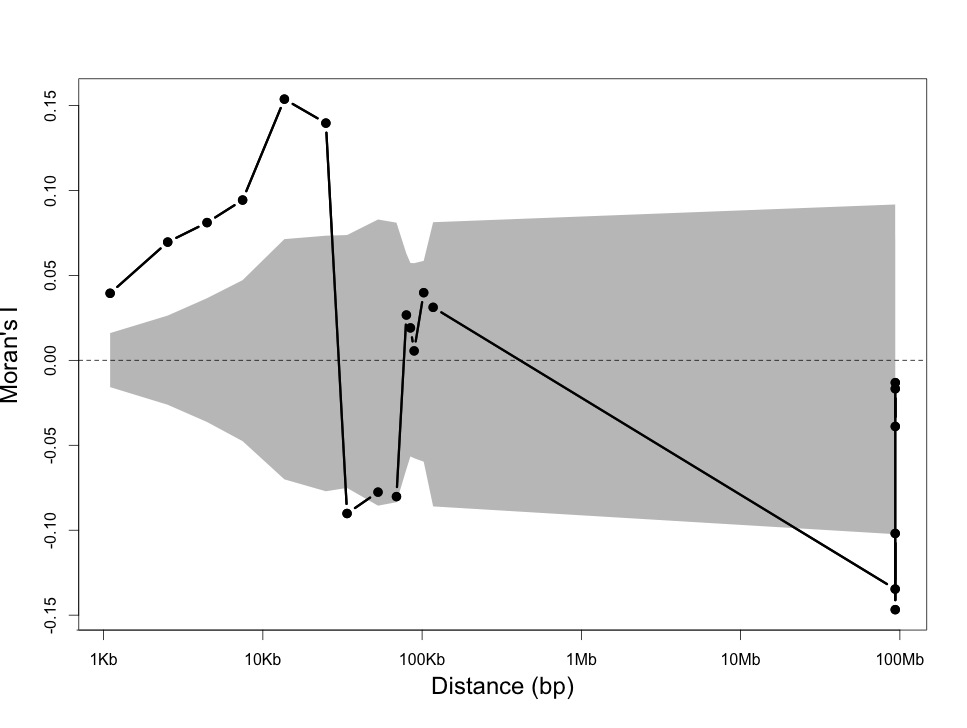
\includegraphics[width=1\textwidth]{Suppl_Chr02_Rspagedi.jpeg}
\caption{Measure of Moran's I for Chromosome 2.  Gray areas show the confidence interval, calculated using permutations of genetic distance.}
\label{Supp_SpagediChr02}    
\end{figure}

\begin{figure}[h!]
% For two-column wide figures use
% Use the relevant command to insert your figure file.
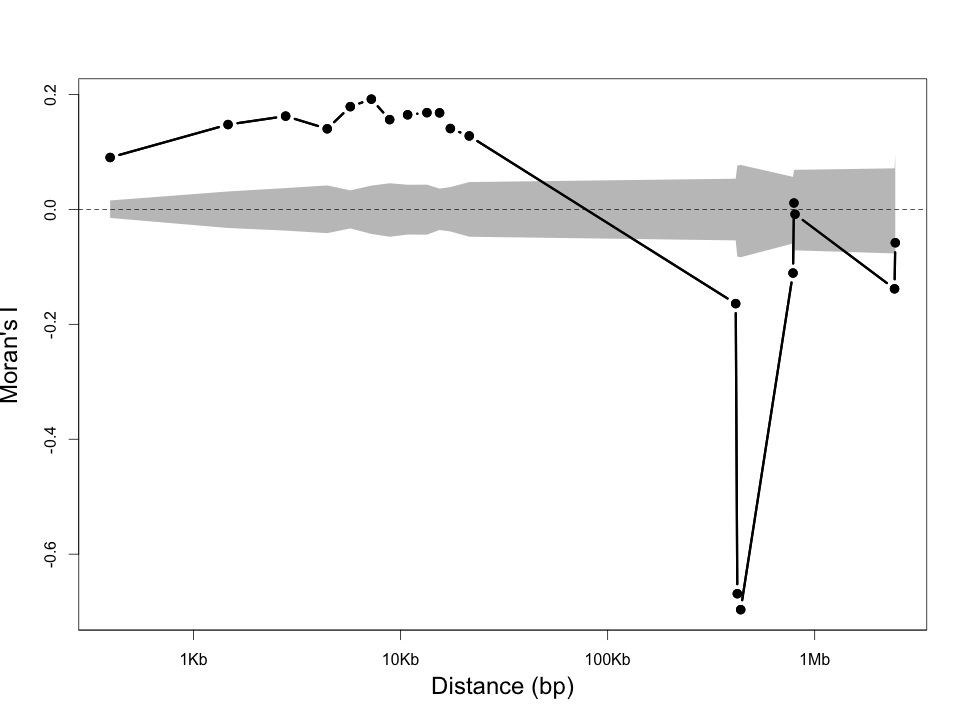
\includegraphics[width=1\textwidth]{Suppl_Chr05_Rspagedi.jpeg}
\caption{Measure of Moran's I for Chromosome 5.  Gray areas show the confidence interval, calculated using permutations of genetic distance.}
\label{Supp_SpagediChr05}    
\end{figure}

\begin{figure}[h!]
% For two-column wide figures use
% Use the relevant command to insert your figure file.
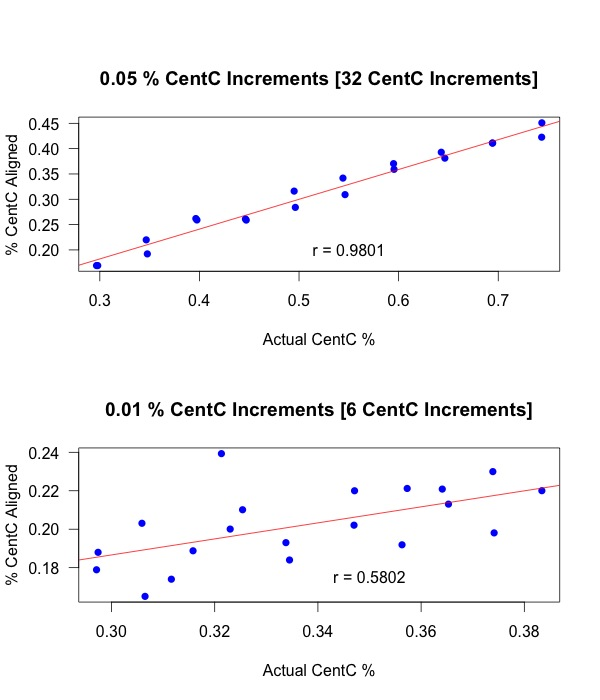
\includegraphics[width=1\textwidth]{AccuracyTest_2graphs.jpeg}
\caption{Graphs showing our ability to capture changes in CentC repeat abundance under constant genome size.  We simulated 10 Mb of DNA with varying CentC content and  simulated Illumina reads from the DNA.  Reads were mapped with our Mosaik pipeline, and several simulations at each percentage of genomic content were performed.}
\label{Supp_Accuracy}    
\end{figure}

\clearpage

\begin{table}[h!]
\caption{CentC Occurence Count In Maize RefGenv2}
\label{supp.occurence}       % Give a unique label
% For LaTeX tables use
\begin{tabular}{ll}
\hline\noalign{\smallskip}
Occurrences &  Number of CentC's\\
\noalign{\smallskip}\hline\noalign{\smallskip}				
1	&8259\\
2	&1233\\
3	&263\\
4	&89\\
5	&31\\
6	&13\\
7	&7\\
8	&0\\
9	&0\\
10	&1\\
\noalign{\smallskip}\hline
\end{tabular}
\end{table}


% For tables use
\begin{table}[h!]
\caption{PacBio Read Counts and Tandem CentC}
\label{supp.pacbio}       % Give a unique label
% For LaTeX tables use
\begin{tabular}{llll}
\hline\noalign{\smallskip}
Maize Line & Reads over 600 bp & Reads with $\geq 4$ CentC & \% Reads Showing Tandem CentC \\
\noalign{\smallskip}\hline\noalign{\smallskip}				
B73	& 237995	& 30	& 0.030252736	\\
\emph{luxurians}		&156964	&	79	&	0.050330012	\\
\emph{mexicana}	 	&141939 	&	150	&	0.1056792	\\
\emph{parviglumis}	&227050	& 89		&	0.039198414	\\
\noalign{\smallskip}\hline
\end{tabular}
\end{table}

% For tables use
\begin{table}[h!]
\caption{ChIP Reads mapping to Unassembled from different Oat-Maize Addition (OMA) Lines.  Reads were mapped using Bowtie2 \citep{langmead2012fast} with the paramater -very sensitive-local.}\label{supp.gaby}       % Give a unique label

% For LaTeX tables use
\begin{tabular}{llll}
\hline\noalign{\smallskip}
File Key & Maize Chr & Percent Reads Aligning to Unassembled BACs\\
\noalign{\smallskip}\hline\noalign{\smallskip}				
JJ1BU (OMA 6.34) & 6 & 21.35\\
JJ1BR (OMA 1.36) & 1 & 15.56\\
JJ1CF (OMA 9.41) & 9 & 6.16\\
JJ1CH (OMA 8.05) & 8 & 6.69\\
JJ1CG (OMA 10.26) & 10 & 9.21\\
JJ1CI (OMA 8.05) & 8 & 8.5\\
\noalign{\smallskip}\hline
\end{tabular}
\end{table}

\clearpage
 \begin{longtable}[c]{|c|c|c|c|c|c|c|c|c|c|c|}
 \caption{Hierarchical clustering group assignment for copies of CentC, sorted by chromosome.  The number of CentC's from each chromosome is represented in the table.\label{long}}\\ 
\hline

\hline
Group & Chr01 & Chr02 & Chr03 & Chr04 & Chr05 & Chr06 & Chr07 & Chr08 & Chr09 & Chr10\\
\hline
\endfirsthead

\multicolumn{1}{c}{Table \ref{long} Continued}\\
\hline
Group & Chr01 & Chr02 & Chr03 & Chr04 & Chr05 & Chr06 & Chr07 & Chr08 & Chr09 & Chr10\\ 
\hline
\endhead 
 
1 & 59 & 10 & 19 & 15 & 28 & 0 & 101 & 31 & 23 & 51\\
2 & 98 & 0 & 0 & 0 & 1 & 0 & 1 & 0 & 1 & 0\\
3 & 149 & 0 & 0 & 0 & 0 & 0 & 1 & 0 & 1 & 1\\
4 & 125 & 45 & 105 & 64 & 72 & 4 & 494 & 117 & 155 & 303\\
5 & 6 & 0 & 0 & 0 & 0 & 0 & 0 & 0 & 0 & 0\\
6 & 1 & 0 & 1 & 0 & 0 & 0 & 0 & 0 & 0 & 0\\
7 & 234 & 0 & 0 & 0 & 0 & 0 & 0 & 0 & 0 & 0\\
8 & 0 & 0 & 0 & 1 & 0 & 0 & 427 & 0 & 0 & 4\\
9 & 0 & 0 & 0 & 0 & 0 & 0 & 0 & 1 & 28 & 81\\
10 & 0 & 0 & 0 & 0 & 0 & 0 & 0 & 0 & 152 & 38\\
11 & 0 & 0 & 0 & 0 & 0 & 0 & 91 & 0 & 0 & 0\\
12 & 242 & 33 & 115 & 0 & 0 & 0 & 8 & 2 & 0 & 1\\
13 & 0 & 0 & 0 & 0 & 0 & 0 & 0 & 0 & 0 & 0\\
14 & 20 & 2 & 17 & 0 & 7 & 0 & 340 & 2 & 3 & 0\\
15 & 28 & 0 & 0 & 0 & 0 & 0 & 0 & 0 & 0 & 0\\
16 & 65 & 0 & 0 & 0 & 0 & 0 & 0 & 0 & 0 & 0\\
17 & 2 & 0 & 0 & 0 & 0 & 0 & 0 & 0 & 0 & 0\\
18 & 113 & 0 & 0 & 0 & 0 & 0 & 0 & 0 & 0 & 0\\
19 & 225 & 0 & 0 & 0 & 0 & 0 & 0 & 0 & 0 & 0\\
20 & 135 & 0 & 0 & 0 & 0 & 0 & 0 & 0 & 0 & 0\\
21 & 200 & 62 & 104 & 0 & 0 & 0 & 1 & 0 & 1 & 0\\
22 & 0 & 0 & 0 & 0 & 8 & 0 & 122 & 0 & 0 & 0\\
23 & 7 & 0 & 0 & 3 & 0 & 0 & 98 & 205 & 123 & 3\\
24 & 17 & 0 & 89 & 0 & 0 & 0 & 0 & 0 & 0 & 0\\
25 & 0 & 1 & 0 & 0 & 0 & 0 & 198 & 0 & 0 & 0\\
26 & 11 & 64 & 22 & 0 & 0 & 0 & 0 & 0 & 0 & 0\\
27 & 6 & 0 & 140 & 47 & 0 & 0 & 0 & 0 & 0 & 0\\
28 & 0 & 0 & 169 & 47 & 0 & 0 & 0 & 0 & 0 & 0\\
29 & 0 & 0 & 0 & 0 & 0 & 0 & 0 & 0 & 0 & 151\\
30 & 0 & 0 & 0 & 66 & 283 & 0 & 1 & 0 & 0 & 0\\
31 & 0 & 0 & 0 & 87 & 202 & 0 & 0 & 0 & 0 & 0\\
32 & 0 & 0 & 0 & 0 & 25 & 0 & 0 & 0 & 0 & 0\\
33 & 0 & 0 & 0 & 0 & 0 & 12 & 55 & 0 & 0 & 0\\
34 & 0 & 0 & 0 & 0 & 2 & 16 & 213 & 0 & 0 & 0\\
35 & 0 & 0 & 0 & 0 & 0 & 0 & 56 & 0 & 0 & 0\\
36 & 0 & 0 & 0 & 0 & 0 & 0 & 217 & 0 & 0 & 0\\
37 & 0 & 0 & 0 & 0 & 0 & 0 & 25 & 0 & 0 & 0\\
38 & 0 & 0 & 0 & 0 & 3 & 0 & 248 & 1 & 19 & 1\\
39 & 0 & 0 & 0 & 0 & 0 & 0 & 60 & 80 & 0 & 0\\
40 & 0 & 0 & 0 & 0 & 0 & 0 & 182 & 0 & 0 & 0\\ 
41 & 0 & 0 & 0 & 0 & 0 & 0 & 90 & 0 & 0 & 0\\  \hline
42 & 0 & 0 & 0 & 0 & 0 & 0 & 58 & 0 & 0 & 0\\
43 & 0 & 0 & 0 & 0 & 0 & 0 & 87 & 0 & 0 & 0\\
44 & 0 & 0 & 0 & 0 & 0 & 0 & 22 & 135 & 1 & 0\\
45 & 0 & 0 & 0 & 0 & 0 & 0 & 0 & 85 & 98 & 0\\
46 & 0 & 0 & 0 & 0 & 0 & 0 & 0 & 0 & 150 & 1\\
47 & 0 & 0 & 0 & 0 & 0 & 0 & 0 & 0 & 0 & 254\\
48 & 0 & 0 & 0 & 0 & 0 & 0 & 0 & 0 & 70 & 0\\
49 & 0 & 0 & 0 & 0 & 0 & 0 & 0 & 0 & 193 & 1\\
50 & 0 & 0 & 0 & 0 & 0 & 0 & 0 & 0 & 93 & 0\\
51 & 0 & 0 & 0 & 0 & 0 & 0 & 0 & 0 & 2 & 62\\
52 & 0 & 0 & 0 & 0 & 0 & 0 & 2 & 0 & 0 & 311\\
53 & 0 & 0 & 0 & 0 & 0 & 0 & 0 & 0 & 0 & 168\\
54 & 0 & 0 & 0 & 0 & 0 & 0 & 0 & 0 & 0 & 112\\
55 & 0 & 0 & 0 & 0 & 0 & 0 & 0 & 0 & 0 & 42\\
56 & 0 & 0 & 0 & 0 & 0 & 0 & 2 & 0 & 0 & 226\\
57 & 0 & 0 & 0 & 0 & 0 & 0 & 0 & 0 & 0 & 66\\
58 & 0 & 0 & 0 & 0 & 0 & 0 & 0 & 0 & 0 & 56\\
\bottomrule
\end{longtable}

\clearpage
\begin{table}[h!]
\caption{Number of clusters in each subgenome under varying criteria for distances apart.  Minimum cluster size is 10,000 bp, though trends remain the same under different mininum cluster sizes.}\label{supp.adjustclust} 
% For LaTeX tables use
\begin{tabular}{ccccccc}
\hline\noalign{\smallskip}
Distance ( bp) &  Unassigned  bp &  Clusters Unassigned &  Subgenome1  bp &  Clusters Subgenome1 & Subgenome2  bp &  Clusters Subgenome2 \\\noalign{\smallskip}\hline\noalign{\smallskip}				
1000 & 96504 & 6 & 829419 & 39 & 92126 & 7\\
2000 & 109482 & 7 & 925028 & 43 & 115538 & 7\\
3000 & 128492 & 8 & 969892 & 44 & 117094 & 7\\
4000 & 128492 & 8 & 994104 & 41 & 124020 & 7\\
5000 & 128492 & 8 & 1026845 & 40 & 136025 & 6\\
6000 & 134203 & 8 & 1054805 & 39 & 140679 & 6\\
7000 & 134203 & 8 & 1069516 & 38 & 140679 & 6\\
8000 & 134203 & 7 & 1139270 & 36 & 140679 & 4\\
9000 & 142786 & 7 & 1162918 & 37 & 147864 & 4\\
10000 & 142786 & 7 & 1179529 & 36 & 149125 & 4\\
11000 & 144185 & 7 & 1198451 & 36 & 149125 & 4\\
12000 & 144185 & 6 & 1203008 & 34 & 149125 & 4\\
13000 & 145273 & 6 & 1210187 & 32 & 149125 & 4\\
14000 & 145273 & 6 & 1210329 & 31 & 149125 & 4\\
15000 & 145273 & 6 & 1215760 & 30 & 149125 & 4\\
16000 & 145273 & 5 & 1224106 & 27 & 152385 & 4\\
17000 & 145273 & 5 & 1224106 & 25 & 152385 & 4\\
18000 & 146060 & 5 & 1224106 & 25 & 157135 & 4\\
19000 & 152703 & 5 & 1229229 & 25 & 157135 & 4\\
20000 & 163555 & 6 & 1234836 & 25 & 157135 & 3\\
\noalign{\smallskip}\hline
\label{tab:suppvartandem} 
\end{tabular}
\end{table}

\end{document}

